\documentclass[../main.tex]{subfiles}
\begin{document}
\subsection{沉降與浮選，Settling and Floating}
\begin{itemize}
  \item Settling，沉降，$\rho_P > \rho$
  \item Floating，浮選，$\rho_P < \rho$
  \item 求出顆粒速度隨時間關係，$\vec{\bm v}(t)$，由牛頓運動定律計算
  \begin{equation}
    \begin{cases}
      \sum F = 0 & \implies v,\quad (\text{steady state}) \\
      \sum F \neq 0 & \implies \sum F = m\vec{\bm a}(t) = m\frac{d\vec{\bm v}(t)}{dt}
    \end{cases}
  \end{equation}
  \item 力的來源
  \begin{itemize}
    \item 重力(Gravity Force)
    \begin{equation}
      F_g = mg = \rho_P V_P g \label{eq:gravity_force}
    \end{equation}
    \item 浮力(Buoyancy Force)\\
    排開液體的重力
    \begin{equation}
      m_fg = \rho_f V_f g = \rho_f V_P g = \rho_f\frac{m}{\rho_P} g \label{eq:buoyancy_force}
    \end{equation}
    P.S. 將(\ref{eq:buoyancy_force})除以(\ref{eq:gravity_force})，可得相對密度
    \begin{equation}
      \frac{F_b}{F_g} = \frac{\rho_f}{\rho_P},\quad \implies F_b = F_g \frac{\rho_f}{\rho_P} \label{eq:relative_density}
    \end{equation}
    \item 阻力(Drag Force)\\
    有一個Drag Coefficient $C_D$，為無因次群\\
    定義式
    \begin{equation}
      C_D = \frac{\text{Drag Force}}{\text{inertial force}} = \frac{F_D/A_P}{\frac{1}{2}\rho v^2} \label{eq:drag_coefficient_definition}
    \end{equation}
    其中$A_P$為顆粒投影面積(Perpendicular Area)\\
    也就是顆粒的最大截面積\\
    故球體的$A_P = \pi R^2$
    P.S. 流力與單操對慣性力的定義不同
    \begin{itemize}
      \item 流力:
      \begin{equation}
        \frac{F}{A} = \frac{\vec{\bm P}(\text{(動量)})}{
          tA
        } = \frac{m\cdot v}{tA} = \frac{\dot m v}{A} = \frac{(\rho \vec{\bm v}A)\vec{\bm v}}{A} 
        = \rho \vec{\bm v}\vec{\bm v}
      \end{equation}
      \item 單操:
      \begin{equation}
        \frac{F}{A} = \frac{\text{KE(動能)}/L}{A} = \frac{\frac{1}{2}mv^2}{V} = \frac{1}{2}\rho v^2
      \end{equation}
    \end{itemize}
  \end{itemize}
  \item 沉降的力平衡:
  \begin{align}
    \frac{d}{dt}(mv) &= F_g - F_b - F_D \\
    m\frac{dv}{dt} &= mg - mg \frac{\rho}{\rho_P} - C_D \frac{1}{2}\rho v^2 A_P 
  \end{align}
  而當粒子達到力平衡時，$dv/dt = 0$，可得終端速度(Terminal Velocity)$v_t$\\
  而終端速度的公式，任何形狀都可使用
  \begin{equation}
    \boxed{v_t = \sqrt{\frac{2\rho(\rho_p-\rho)m}{A_p \rho_p C_D \rho}}}
  \end{equation}
  當顆粒為球體時
  \begin{align}
    &V_p = \frac{\pi}{2}R_P^3 = \frac{\pi}{3}\left(
      \frac{D_P}{2}^3
    \right) = \frac{\pi}{6}D_P^3 \\
    &m = \rho_P V_P = \rho_P \frac{\pi}{6}D_P^3 \\
    &A_P = \pi R_P^2 = \frac{\pi}{4}D_P^2 \\
    &\therefore v_t = \sqrt{\frac{4(\rho_P - \rho)g D_P}{3 C_D \rho}} 
  \end{align}
  由上式可知，影響物體終端速度的因素有四
  \begin{enumerate}
    \item 密度差：$(\rho_P - \rho) \propto v_t$
    \item 顆粒直徑：$D_P \propto v_t$
    \item 流體密度：$\rho \propto v_t^{-1}$
    \item 阻力係數：$C_D \propto v_t^{-1}$
  \end{enumerate}
  \item 浮選的力平衡:
  \begin{equation}
    \frac{d}{dt}(mv) = = F_g + F_b - F_D
  \end{equation}
  其餘同沉降\\
  最後會得到終端速率:
  \begin{equation}
    v_t = \sqrt{\frac{4(\rho - \rho_p)\cdot g D_P}{3C_D\rho}}
  \end{equation}
  \item Particle Reynolds Number，顆粒雷諾數
  \begin{equation}
    Re_P = \frac{\rho v_t D_P}{\mu}
  \end{equation}
  \item 沉降的四個階段
  \begin{itemize}
    \item $\boxed{\text{Re}_P\leq 1}$，Creeping flow, stokes law:
    \begin{equation}
      F_D = 3\pi \mu D_p v_\infty \leftrightarrow  F_D = 3\pi \mu D_P v_t
    \end{equation}
    分別為流體力學與單操的定義式\\
    用於Settling時
    \begin{align}
      C_D &= \frac{F_D/A_P}{\frac{1}{2}\rho v_t^2} \nonumber\\
      &= \frac{3\pi \mu D_P v_t/\frac{\pi}{4}D_P^2}{\frac{1}{2}\rho v_t^2} \nonumber\\
      &= \frac{24\mu}{\rho v_t D_P} \nonumber\\
      &= \frac{24}{Re_P}
    \end{align}
    將上式以$\log C_D$為縱軸，$\log Re_P$為橫軸繪圖，可得一條直線，斜率$=-1$\\
    而截距為$\log 24$\\
    而此時的終端速度為
    \begin{equation}
      v_t = \frac{(\rho_P - \rho)g D_P^2}{18\mu}
    \end{equation}
    P.S. 此時的終端速度與\fbox{黏度成反比}
    \item $\boxed{1 < \text{Re}_P < 1000}$\\
    過度區間，只能依靠經驗式\\
    或查圖得到$C_D$後，再帶入終端速度公式
    \begin{equation}
      v_t = \sqrt{\frac{4(\rho_P - \rho)g D_P}{3 C_D \rho}}
    \end{equation}
    \item $\boxed{1000 < \text{Re}_P < 2\times 10^5}$\\
    牛頓流區間(Newtonian flow Regime)
    \begin{equation}
      \boxed{\frac{F_D}{A_P} \propto v_t^2 \implies C_D = \text{constant} \approx 0.44}
    \end{equation}
    又稱為牛頓阻力定律(Newton's Drag Law)\\
    在以$\log C_D$為縱軸，$\log Re_P$為橫軸繪圖中，會呈現一個水平線\\
    而此時的終端速度為
    \begin{equation}
      v_t = \sqrt{\frac{4(\rho_P - \rho)g D_P}{3\cdot 0.44 \cdot \rho}}
       = 1.75\sqrt{\frac{(\rho_P - \rho)g D_P}{\rho}}
    \end{equation}
    \fbox{與黏度無關，由慣性力主導}
    \item $\boxed{\text{Re}_P > 2\times 10^5}$\\
    因為\fbox{分離點向後移動}，會瞬間下掉\\
    而所謂的分離點，是指流體從物體表面分離的點\\
    此時分離點超過了90度，會產生渦流，使得阻力下降
  \end{itemize}
  \begin{figure}[H]
    \centering
    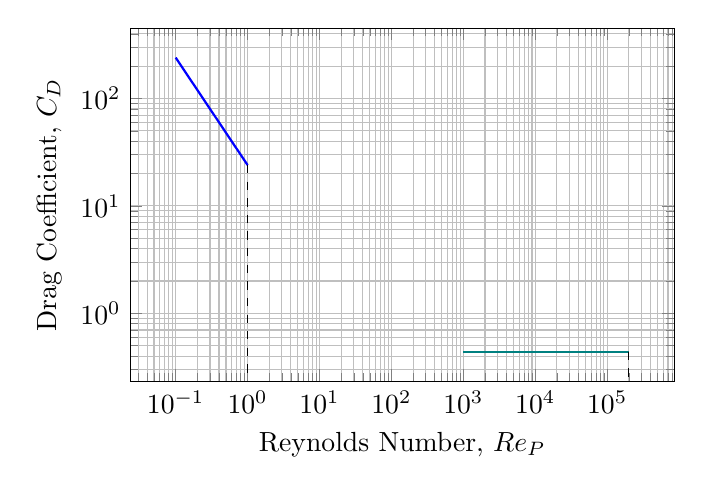
\begin{tikzpicture}
      \begin{loglogaxis}[
        xlabel={Reynolds Number, $Re_P$},
        ylabel={Drag Coefficient, $C_D$},
        grid=both,
        width=0.7\textwidth,
        height=0.5\textwidth,
        domain=0.1:1000000,
        samples=100
      ]
        \addplot[blue, thick, domain=0.1:1] {24/x};
        \addplot[teal, thick, domain=1000:200000] {0.44};
        \draw[dashed] (axis cs:1,24) -- (axis cs:1,0.1);
        \draw[dashed] (axis cs:1000,0.024) -- (axis cs:1000,0.1);
        \draw[dashed] (axis cs:200000,0.44) -- (axis cs:200000,0.1);
      \end{loglogaxis}
    \end{tikzpicture}
    \caption{顆粒阻力係數與雷諾數關係圖}
  \end{figure}
  \item 沉降的類型:
  \begin{itemize}
    \item Free settling，自由沉降\\
    顆粒濃度低時，顆粒與顆粒之間距離遠\\
    顆粒沉降過程，不受到其他顆粒影響\\
    只受到顆粒本身所受重力、浮力與阻力影響
    \item Hindered settling，受阻沉降\\
    當顆粒濃度高時，因為顆粒與顆粒之間距離太近\\
    顆粒沉降過程，會受到其他顆粒影響，而這種影響為負面的\\
    因此通常受阻沉降的速度會比自由沉降來得慢
  \end{itemize}
  \item 分離點\\
  流體流過曲面時，會有兩個Drag Force
  \begin{itemize}
    \item Skin Friction Drag，表面摩擦阻力\\
    流體與物體表面之間的黏滯作用所產生的阻力
    \item Form Drag，形狀阻力\\
    物體形狀造成的壓力差所產生的阻力
  \end{itemize}
  流體流過球體的位置為0度，則大約在80度左右會有分離點\\
  而分離點到邊界層的曲率是與小於分離點的邊界層曲率相反的\\
  而分離點則剛好是反曲點\\
  而過了分離點，邊界層內會有逆流出現\\
  因此產生漩渦(eddy)，而漩渦會增加阻力\\
  但當速度夠快時($Re_P > 2\times 10^5$)，分離點會往後移到90度以上，約110度\\
  此時能產生逆流的區域變小，阻力也瞬間變小
\end{itemize}
\end{document}
